\documentclass[10pt,aspectratio=169]{beamer}
\usetheme{Madrid}
\usepackage{amsmath,booktabs,pgfplots}
\pgfplotsset{compat=1.18}

\title{Experiment Results And Evidence}
\author{Speaker}
\date{\today}

\begin{document}
\begin{frame}\titlepage\end{frame}

\begin{frame}{Experimental Question}
  \begin{itemize}
    \item Hypothesis.
    \item Dataset or benchmark.
    \item Metric and protocol.
  \end{itemize}
\end{frame}

\begin{frame}{Main Plot}
  \centering
  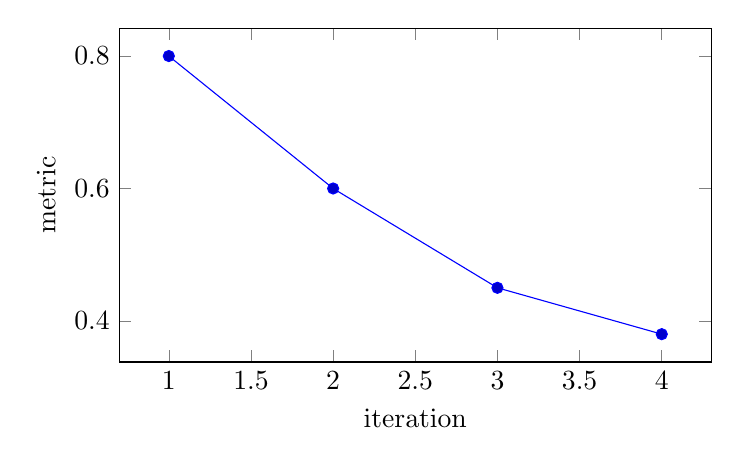
\begin{tikzpicture}
    \begin{axis}[width=.75\textwidth,height=.48\textwidth,xlabel={iteration},ylabel={metric}]
      \addplot coordinates {(1,0.8) (2,0.6) (3,0.45) (4,0.38)};
    \end{axis}
  \end{tikzpicture}
\end{frame}

\begin{frame}{Ablation Table}
  \begin{tabular}{lrr}
    \toprule
    Variant & Score & Cost \\
    \midrule
    Baseline & -- & -- \\
    Proposed & -- & -- \\
    Without component & -- & -- \\
    \bottomrule
  \end{tabular}
\end{frame}

\begin{frame}{Reproducibility Checklist}
  Code commit, seed, hardware, data split, and evaluation script.
\end{frame}
\end{document}
